\documentclass[../main.tex]{subfiles}
\begin{document}
本章主要参考\cite{euclid,geometry}。

% Reference: https://math.osu.edu/sites/math.osu.edu/files/ceva-menelaus.pdf
% References: https://mathworld.wolfram.com/Exradius.html
% https://mathworld.wolfram.com/Orthocenter.html
% https://mathworld.wolfram.com/Nine-PointCircle.html
% https://mathworld.wolfram.com/BretschneidersFormula.html
% Pitot converse: https://doi.org/10.1017/mag.2021.7
本章讨论 Euclid 平面几何。角度统一使用弧度；三角函数恒等式见初等数学章。未特别说明时，长度为正，三角形及多边形非退化。
\section{基本图形与相似}
\subsection{角、平行线与多边形}\index{角、平行线与多边形|hyperpage}
三角形内角和为 $\pi$；平行线被截时同位角、内错角相等，同旁内角互补。凸 $n$ 边形（$n\ge3$）满足
\[
\sum_{i=1}^n\alpha_i=(n-2)\pi,\qquad
\text{对角线条数}=\frac{n(n-3)}2.
\]
沿边界同向转动时，凸多边形外角和为 $2\pi$；正 $n$ 边形的内角为 $(n-2)\pi/n$，中心角为 $2\pi/n$。
\subsection{全等、相似与平行截线}\index{全等、相似与平行截线|hyperpage}
三角形全等的常用判据为 SSS、SAS、ASA、AAS；直角三角形还可用斜边与一直角边（HL）。SAS 中的角必须是两边的夹角。
三角形相似可由两角对应相等、三边对应成比例，或两边对应成比例且夹角相等判定。相似比为 $k>0$ 时，
\[
\frac{P_2}{P_1}=k,\qquad\frac{S_2}{S_1}=k^2.
\]
若 $D\in AB,E\in AC$ 且 $DE\parallel BC$，则
\[
\frac{AD}{AB}=\frac{AE}{AC}=\frac{DE}{BC},\qquad
\frac{AD}{DB}=\frac{AE}{EC}\quad(D,E\text{ 均为内点}).
\]
仅有两边及非夹角相等，通常不能保证全等。
\subsection{正多边形的边长、半径与面积}\index{正多边形的边长、半径与面积|hyperpage}
设正 $n$ 边形（$n\ge3$）的边长为 $a$，外接圆半径为 $R$，内切圆半径为 $\rho$，周长为 $P$，面积为 $S$，则
\begin{align*}
a&=2R\sin\frac\pi n, &
\rho&=R\cos\frac\pi n=\frac{a}{2\tan(\pi/n)},\\
P&=na, & S&=\frac12P\rho=\frac{na^2}{4\tan(\pi/n)}
=\frac n2R^2\sin\frac{2\pi}{n}.
\end{align*}
两个顶点沿边界相隔 $k$ 条边时，对应的弦长为
\[
d_k=2R\sin\frac{k\pi}{n},\qquad
1\le k\le\left\lfloor\frac n2\right\rfloor.
\]
$k=1$ 对应边长；$k\ge2$ 对应对角线。这里 $\rho$ 是正多边形中心到任意一边的距离。
\section{三角形}
\subsection{边角关系、勾股定理与面积}\index{边角关系、勾股定理与面积|hyperpage}
记 $a=BC,b=CA,c=AB$，对应内角为 $A,B,C$，半周长 $s=(a+b+c)/2$，面积为 $\Delta$，则
\begin{gather*}
|b-c|<a<b+c,\qquad a^2=b^2+c^2-2bc\cos A,\\
\frac a{\sin A}=\frac b{\sin B}=\frac c{\sin C}=2R,\\
\Delta=\frac12ah_a=\frac12bc\sin A
=\sqrt{s(s-a)(s-b)(s-c)}=rs=\frac{abc}{4R}.
\end{gather*}
$R,r$ 分别为外接圆、内切圆半径。$A=\pi/2$ 时有 $a^2=b^2+c^2$；反之该等式也判定 $A$ 为直角。正三角形边长 $a$ 时，$\Delta=\sqrt3a^2/4$。
\subsection{半角公式与旁切圆}\index{半角公式与旁切圆|hyperpage}
沿用 $a=BC,b=CA,c=AB$、$s=(a+b+c)/2$、面积 $\Delta$ 的约定，则
\begin{align*}
\sin\frac A2&=\sqrt{\frac{(s-b)(s-c)}{bc}}, &
\cos\frac A2&=\sqrt{\frac{s(s-a)}{bc}},\\
\tan\frac A2&=\sqrt{\frac{(s-b)(s-c)}{s(s-a)}}=\frac r{s-a}.
\end{align*}
$B,C$ 的对应公式由循环置换得到。三角形内角的半角位于 $(0,\pi/2)$，故上述根式均取正值。
对边 $a,b,c$ 的旁切圆半径分别为
\[
r_a=\frac\Delta{s-a},\qquad r_b=\frac\Delta{s-b},\qquad
r_c=\frac\Delta{s-c}.
\]
它们与内切圆、外接圆半径满足
\begin{align*}
\frac1{r_a}+\frac1{r_b}+\frac1{r_c}&=\frac1r, &
r_ar_br_c&=rs^2,\\
rr_ar_br_c&=\Delta^2, & r_a+r_b+r_c&=4R+r.
\end{align*}
例如乘积公式可由 Heron 公式直接得到：
\[
r_ar_br_c=\frac{\Delta^3}{(s-a)(s-b)(s-c)}=s\Delta=rs^2.
\]
\subsection{直角三角形的射影定理}\index{直角三角形的射影定理|hyperpage}
设 $\angle A=\pi/2$，$AD\perp BC$，垂足 $D$ 在斜边内部。记 $BC=a$、$CA=b$、$AB=c$，以及 $BD=u$、$DC=v$、$AD=h$，则
\begin{align*}
a&=u+v, & c^2&=au, & b^2&=av, & h^2&=uv,\\
h&=\frac{bc}{a}, & \frac1{h^2}&=\frac1{b^2}+\frac1{c^2}, &
R&=\frac a2, & r&=\frac{b+c-a}{2}.
\end{align*}
\par\begin{samepage}
\begin{center}
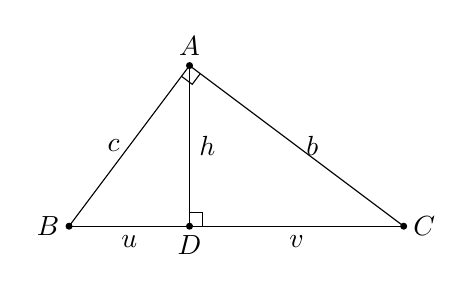
\begin{tikzpicture}[scale=0.85]
\coordinate (B) at (0,0);\coordinate (C) at (5,0);
\coordinate (D) at (1.8,0);\coordinate (A) at (1.8,2.4);
\draw (B)--node[left]{$c$}(A)--node[right]{$b$}(C);
\draw (B)--node[below]{$u$}(D)--node[below]{$v$}(C);
\draw (A)--node[right]{$h$}(D);
\draw (1.8,0.2)--(2,0.2)--(2,0);
\draw (1.68,2.24)--(1.84,2.12)--(1.96,2.28);
\fill (A) circle(1.5pt) node[above]{$A$};
\fill (B) circle(1.5pt) node[left]{$B$};
\fill (C) circle(1.5pt) node[right]{$C$};
\fill (D) circle(1.5pt) node[below]{$D$};
\end{tikzpicture}
\end{center}
图中整条斜边长为 $a=u+v$；$c^2$ 对应投影 $u$，$b^2$ 对应投影 $v$，不可交换。
\par\end{samepage}
\subsection{中线、角平分线、高与Stewart公式}\index{中线、角平分线、高与Stewart公式|hyperpage}
从 $A$ 引出的中线长 $m_a$、内角平分线长 $\ell_a$ 和高 $h_a$ 满足
\[
m_a=\frac12\sqrt{2b^2+2c^2-a^2},\qquad
\ell_a=\frac{2bc\cos(A/2)}{b+c}
=\sqrt{bc\left(1-\frac{a^2}{(b+c)^2}\right)},\qquad h_a=\frac{2\Delta}a.
\]
若 $AD$ 为内角平分线、$D\in BC$，则 $BD/DC=c/b$。更一般地，设 $BD=m,DC=n,AD=d$，$D$ 在边内，Stewart 公式为
\[
b^2m+c^2n=a(d^2+mn),\qquad a=m+n.
\]
\begin{center}
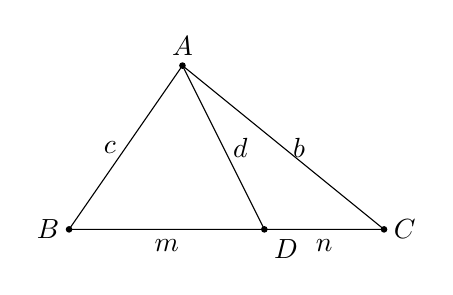
\begin{tikzpicture}[scale=0.8]
\coordinate (A) at (1.8,2.6);\coordinate (B) at (0,0);
\coordinate (C) at (5,0);\coordinate (D) at (3.1,0);
\draw (A)--node[left]{$c$}(B)--node[below]{$m$}(D)--node[below]{$n$}(C)--node[right]{$b$}(A);
\draw (A)--node[right]{$d$}(D);
\fill (A) circle(1.5pt) node[above]{$A$};\fill (B) circle(1.5pt) node[left]{$B$};
\fill (C) circle(1.5pt) node[right]{$C$};\fill (D) circle(1.5pt) node[below right]{$D$};
\end{tikzpicture}
\end{center}
图中 $D$ 是任意边内点；只有角平分线情形才额外满足 $m/n=c/b$。
\subsection{中线与重心的距离关系}\index{中线与重心的距离关系|hyperpage}
若 $M$ 为 $BC$ 中点，阿波罗尼斯公式为
\[
AB^2+AC^2=2AM^2+\frac12BC^2.
\]
三条中线长及重心 $G$ 到各顶点的距离满足
\begin{align*}
m_a^2+m_b^2+m_c^2&=\frac34(a^2+b^2+c^2),\\
GA^2+GB^2+GC^2&=\frac{a^2+b^2+c^2}{3}.
\end{align*}
\par\begin{samepage}
对任意平面点 $P$，有
\[
PA^2+PB^2+PC^2=3PG^2+\frac{a^2+b^2+c^2}{3}.
\]
因此距离平方和的最小值为 $(a^2+b^2+c^2)/3$，且仅在 $P=G$ 时取得。
\par\end{samepage}
\subsection{重心、内心、外心与垂心}\index{重心、内心、外心与垂心|hyperpage}
三条中线交于重心 $G$；若 $M$ 为 $BC$ 中点，则 $AG:GM=2:1$。在平面坐标中，
\[
G=\frac{A+B+C}{3},\qquad
I=\frac{aA+bB+cC}{a+b+c},\qquad
r=\frac\Delta s,\quad R=\frac{abc}{4\Delta},\quad r_a=\frac\Delta{s-a}.
\]
点的线性组合按坐标计算。$I$ 为内心；$r_a$ 为对边 $a$ 的旁切圆半径。外心 $O$ 为边的垂直平分线交点，垂心 $H$ 为高线交点。非正三角形的 $O,G,H$ 共线且 $OG:GH=1:2$。
\[
OI^2=R(R-2r),\qquad R\ge2r,
\]
等号当且仅当三角形为正三角形。
\subsection{欧拉线上的向量关系与九点圆}\index{欧拉线上的向量关系与九点圆|hyperpage}
用位置向量表示点，则任意非退化三角形满足
\[
H=A+B+C-2O,\qquad \overrightarrow{OH}=3\overrightarrow{OG}.
\]
中心间距离可由边长和外接圆半径求得：
\[
OH^2=9R^2-(a^2+b^2+c^2),\qquad
OG^2=R^2-\frac{a^2+b^2+c^2}{9}.
\]
这些关系适用于锐角、直角及钝角三角形；正三角形中 $O=G=H$，不再确定唯一的欧拉线。
\par\begin{samepage}
九点圆经过三边中点、三条高在对边所在直线上的垂足，以及 $AH,BH,CH$ 的中点。其圆心 $N$、半径 $R_N$ 为
\[
N=\frac{O+H}{2},\qquad R_N=\frac R2.
\]
直角三角形中，上述九个构造点可能重合，但九点圆仍存在。
\par\end{samepage}
\section{四边形与圆}
\subsection{四边形面积与圆内接四边形}\index{四边形面积与圆内接四边形|hyperpage}
平行四边形面积为 $ah$，梯形面积为 $(a+b)h/2$，这里 $a,b$ 为两底。凸四边形的两对角线长为 $d_1,d_2$、夹角为 $\theta$ 时，
\[
S=\frac12d_1d_2\sin\theta.
\]
凸四边形 $ABCD$ 共圆当且仅当对角互补。共圆时 Ptolemy 公式与 Brahmagupta 公式为
\[
AC\cdot BD=AB\cdot CD+AD\cdot BC,\qquad
S=\sqrt{(s-a)(s-b)(s-c)(s-d)},
\]
其中 $a,b,c,d$ 为顺次边长、$s=(a+b+c+d)/2$。最后的面积公式不能无条件用于一般四边形。
\subsection{一般凸四边形与外切四边形}\index{一般凸四边形与外切四边形|hyperpage}
对凸四边形 $ABCD$，设顺次边长为 $a,b,c,d$，半周长为 $s=(a+b+c+d)/2$，对角 $\alpha=\angle DAB$、$\gamma=\angle BCD$，则 Bretschneider 公式为
\[
S^2=(s-a)(s-b)(s-c)(s-d)
-abcd\cos^2\frac{\alpha+\gamma}{2}.
\]
当 $\alpha+\gamma=\pi$ 时，第二项为零，得到圆内接四边形的 Brahmagupta 公式。
若凸四边形的四条边都与同一内切圆相切，设圆半径为 $\rho$，则
\[
a+c=b+d=s,\qquad S=\rho s.
\]
上述边长等式来自同一点所引的两条切线段相等。Pitot 定理及其逆定理表明：对凸四边形，$a+c=b+d$ 是存在内切圆的充要条件；凸性条件不能省略。
\subsection{弦、切线、弧与扇形}\index{弦、切线、弧与扇形|hyperpage}
圆周角等于其所对弧对应的圆心角的一半；同弧所对圆周角相等，直径所对圆周角为直角。切线垂直于切点处半径。
\par\begin{samepage}
半径为 $R$、对应圆心角为 $\theta$ 时，
\[
\ell_{\text{弧}}=R\theta,\qquad S_{\text{扇形}}=\frac12R^2\theta,
\qquad c_{\text{弦}}=2R\sin(\theta/2)\quad(0\le\theta\le2\pi).
\]
对小弓形取 $0\le\theta\le\pi$，面积为 $R^2(\theta-\sin\theta)/2$。弦长 $c$ 与圆心到弦的距离 $d$ 满足 $d^2+(c/2)^2=R^2$。
\par\end{samepage}
\subsection{弦高与两圆的公切线}\index{弦高与两圆的公切线|hyperpage}
设小弓形的弦长为 $c$，弦高为 $h$（弦中点至小弧中点的距离），则 $0<h\le R$，且
\[
c=2\sqrt{2Rh-h^2},\qquad
R=\frac{c^2}{8h}+\frac h2,\qquad
h=R-\sqrt{R^2-\frac{c^2}{4}}.
\]
设两圆半径为 $R,r>0$、圆心距为 $d$。当 $d>R+r$，两圆外离，两切点之间的公切线段长度分别为
\[
L_{\text{外公切线}}=\sqrt{d^2-(R-r)^2},\qquad
L_{\text{内公切线}}=\sqrt{d^2-(R+r)^2}.
\]
外公切线的两圆心在切线同侧，内公切线的两圆心在切线异侧。以上公式讨论外离的非退化情形；相切时某些切点会重合。
\subsection{两圆的位置关系}\index{两圆的位置关系|hyperpage}
对圆心不同的两圆，记 $d=O_1O_2>0$，半径为 $R,r>0$，则
\[
\begin{array}{c|c}
\text{条件}&\text{位置关系}\\\hline
d>R+r&\text{外离}\\
d=R+r&\text{外切}\\
|R-r|<d<R+r&\text{相交于两点}\\
d=|R-r|&\text{内切}\\
0<d<|R-r|&\text{内含且不相交}
\end{array}
\]
若 $d=0$，则 $R=r$ 时两圆重合，$R\ne r$ 时为不相交的同心圆，不能套用内切判据。
\subsection{圆幂、割线与根轴}\index{圆幂、割线与根轴|hyperpage}
点 $P$ 对圆 $(O,R)$ 的幂为 $\operatorname{Pow}(P)=OP^2-R^2$。若过 $P$ 的直线交圆于 $A,B$，采用该直线上的有向长度，则
\[
\overline{PA}\,\overline{PB}=OP^2-R^2.
\]
$P$ 在圆外且 $PT$ 为切线段时，$PT^2=PA\cdot PB=OP^2-R^2$；$P$ 在圆内时，无向长度满足 $PA\cdot PB=R^2-OP^2$。
两个圆心不同的圆，其等幂点组成一条直线，称根轴；在直角坐标中两圆方程相减即可得到根轴方程。
\section{共线、共点与坐标方法}
\subsection{Ceva与Menelaus定理}\index{Ceva与Menelaus定理|hyperpage}
在非退化三角形 $ABC$ 中，$D,E,F$ 分别位于 $BC,CA,AB$ 的内部，则
\[
AD,BE,CF\text{ 共点}\iff\frac{BD}{DC}\frac{CE}{EA}\frac{AF}{FB}=1.
\]
对三条边所在直线上的非顶点 $D,E,F$，采用有向长度（每条直线上固定同一个正方向），Menelaus 定理为
\[
D,E,F\text{ 共线}\iff
\frac{\overline{BD}}{\overline{DC}}\frac{\overline{CE}}{\overline{EA}}\frac{\overline{AF}}{\overline{FB}}=-1.
\]
若改用无向长度，必须另行检查内外分位置，不能保留有向公式的负号后直接代入正数。
\subsection{三角形式的Ceva定理}\index{三角形式的Ceva定理|hyperpage}
设 $D,E,F$ 分别在 $BC,CA,AB$ 内部，则
\[
AD,BE,CF\text{ 共点}\iff
\frac{\sin\angle BAD}{\sin\angle DAC}
\frac{\sin\angle CBE}{\sin\angle EBA}
\frac{\sin\angle ACF}{\sin\angle FCB}=1.
\]
例如由同高三角形面积之比可得
\[
\frac{BD}{DC}=\frac{c\sin\angle BAD}{b\sin\angle DAC},
\]
其余两式循环置换后相乘即得到上述判据。内点条件保证分母非零；推广到边的延长线时，应重新约定有向角与有向比。
\subsection{面积坐标与重心坐标}\index{面积坐标与重心坐标|hyperpage}
记 $[XYZ]=\tfrac12\det(Y-X,Z-X)$ 为有向面积。对非退化三角形 $ABC$ 和任意平面点 $P$，令
\[
u=\frac{[PBC]}{[ABC]},\qquad
v=\frac{[PCA]}{[ABC]},\qquad
w=\frac{[PAB]}{[ABC]},
\]
则
\[
u+v+w=1,\qquad P=uA+vB+wC.
\]
$P$ 在三角形内部当且仅当 $u,v,w>0$；在三角形及其边界上当且仅当三者非负。
一般的重心坐标写作 $(\lambda:\mu:\nu)$，其中 $\lambda+\mu+\nu\ne0$，对应
\[
P=\frac{\lambda A+\mu B+\nu C}{\lambda+\mu+\nu}.
\]
同时乘以任意非零常数不改变该点。特别地，重心为 $(1:1:1)$，内心为 $(a:b:c)$。
\subsection{平面向量与有向面积}\index{平面向量与有向面积|hyperpage}
对 $u=(u_1,u_2),v=(v_1,v_2)$，定义
\[
u\cdot v=u_1v_1+u_2v_2=|u||v|\cos\theta,\qquad
\det(u,v)=u_1v_2-u_2v_1.
\]
非零向量垂直当且仅当点积为零，平行当且仅当上述二阶行列式为零。
\[
\Delta_{ABC}=\frac12|\det(B-A,C-A)|,\qquad
S_{\text{多边形}}=\frac12\left|\sum_{i=1}^n(x_iy_{i+1}-x_{i+1}y_i)\right|.
\]
多边形顶点须沿边界顺次排列，取 $(x_{n+1},y_{n+1})=(x_1,y_1)$；自交多边形的同一和式表示有向面积。
\subsection{旋转、反射、位似与反演}\index{旋转、反射、位似与反演|hyperpage}
绕原点逆时针转角 $\theta$ 的坐标变换为
\[
x'=x\cos\theta-y\sin\theta,\qquad y'=x\sin\theta+y\cos\theta.
\]
点 $P=(x,y)$ 关于直线 $ax+by+c=0$（$a^2+b^2>0$）的对称点为
\[
P'=P-\frac{2(ax+by+c)}{a^2+b^2}(a,b).
\]
以 $O$ 为中心、比为 $k\ne0$ 的位似为 $P'=O+k(P-O)$，长度按 $|k|$、面积按 $k^2$ 缩放。半径 $\rho>0$ 的反演为
\[
P'=O+\frac{\rho^2}{|P-O|^2}(P-O),\qquad OP\cdot OP'=\rho^2\quad(P\ne O).
\]
反演将不过中心的圆变为圆、过中心的圆变为不过中心的直线；涉及中心的点须单独处理。
\section{平面解析几何}
\subsection{两点距离与线段分点}\index{两点距离与线段分点|hyperpage}
对 $A=(x_1,y_1)$、$B=(x_2,y_2)$，有
\[
AB=\sqrt{(x_2-x_1)^2+(y_2-y_1)^2},\qquad
M=\frac{A+B}{2}.
\]
若 $P$ 内分线段 $AB$，且 $AP:PB=m:n$（$m,n>0$），则
\[
P=\frac{nA+mB}{m+n}
=\left(\frac{nx_1+mx_2}{m+n},\frac{ny_1+my_2}{m+n}\right).
\]
若 $P$ 外分 $AB$ 且无向长度满足 $AP:PB=m:n$，则
\[
P=\frac{mB-nA}{m-n}\quad(m,n>0,\ m\ne n).
\]
内分和外分公式的权重顺序与符号不同；外分比为 $1:1$ 时不存在有限分点。
\subsection{直线、距离与圆}\index{直线、距离与圆|hyperpage}
直线 $Ax+By+C=0$（$A^2+B^2>0$）的法向量为 $(A,B)$。点 $P(x_0,y_0)$ 到直线的距离为
\[
d=\frac{|Ax_0+By_0+C|}{\sqrt{A^2+B^2}}.
\]
非垂直直线的斜率为 $k$，点斜式为 $y-y_0=k(x-x_0)$；两非垂直直线垂直当且仅当 $k_1k_2=-1$。
圆心 $(h,k)$、半径 $r>0$ 的圆为 $(x-h)^2+(y-k)^2=r^2$；在圆上点 $(x_0,y_0)$ 处的切线为
\[
(x_0-h)(x-h)+(y_0-k)(y-k)=r^2.
\]
\subsection{直线夹角与平行线距离}\index{直线夹角与平行线距离|hyperpage}
设直线 $\ell_i:A_ix+B_iy+C_i=0$，$A_i^2+B_i^2>0$（$i=1,2$）。其较小夹角 $\theta\in[0,\pi/2]$ 满足
\[
\cos\theta=
\frac{|A_1A_2+B_1B_2|}
{\sqrt{A_1^2+B_1^2}\sqrt{A_2^2+B_2^2}}.
\]
因此
\begin{align*}
\ell_1\parallel\ell_2\ \text{或重合}
&\iff A_1B_2-A_2B_1=0,\\
\ell_1\perp\ell_2&\iff A_1A_2+B_1B_2=0.
\end{align*}
非垂直情形还可用
\[
\tan\theta=\frac{|A_1B_2-A_2B_1|}{|A_1A_2+B_1B_2|}.
\]
将两条平行线写成相同法向量的形式 $Ax+By+C_1=0$、$Ax+By+C_2=0$ 后，距离为
\[
d=\frac{|C_1-C_2|}{\sqrt{A^2+B^2}}\quad(A^2+B^2>0).
\]
若两个方程的法向量仅成比例，应先归一到同一法向量，再作常数项之差。
\subsection{椭圆、双曲线与抛物线}\index{椭圆、双曲线与抛物线|hyperpage}
以下曲线以坐标轴为对称轴，平移后可将 $x,y$ 替换为 $x-h,y-k$。
\paragraph{椭圆} $a>b>0$，长轴沿 $x$ 轴：
\[
\frac{x^2}{a^2}+\frac{y^2}{b^2}=1,\quad c^2=a^2-b^2,\quad
e=c/a\in(0,1),\quad F_{1,2}=(\pm c,0).
\]
准线为 $x=\pm a/e$，两焦距之和为 $2a$；参数式 $x=a\cos t,y=b\sin t$，面积 $\pi ab$。
\paragraph{双曲线} $a,b>0$，实轴沿 $x$ 轴：
\[
\frac{x^2}{a^2}-\frac{y^2}{b^2}=1,\quad c^2=a^2+b^2,\quad e=c/a>1.
\]
焦点 $(\pm c,0)$，准线 $x=\pm a/e$，渐近线 $y=\pm(b/a)x$，两焦距之差的绝对值为 $2a$。
\paragraph{抛物线} 采用 $y^2=2px$（$p>0$）的约定：焦点 $(p/2,0)$，准线 $x=-p/2$，离心率 $e=1$；参数式 $x=pt^2/2,y=pt$。
\par\begin{samepage}
椭圆与双曲线在曲线上点 $(x_0,y_0)$ 的切线分别为
\[
\frac{xx_0}{a^2}+\frac{yy_0}{b^2}=1,\qquad
\frac{xx_0}{a^2}-\frac{yy_0}{b^2}=1;
\]
抛物线 $y^2=2px$ 的切线为 $yy_0=p(x+x_0)$。易错点：不同教材对抛物线参数 $p$ 的约定可能不同。
\par\end{samepage}
\subsection{直线与圆锥曲线的交点、切线与弦长}\index{直线与圆锥曲线的交点、切线与弦长|hyperpage}
设圆锥曲线由二次方程 $F(x,y)=0$ 给出，参数直线为
\[
P(t)=P_0+t\,v,\qquad v=(v_x,v_y)\ne0.
\]
代入后，若得到 $\alpha t^2+\beta t+\gamma=0$ 且 $\alpha\ne0$，记 $D=\beta^2-4\alpha\gamma$，则
\[
t_{1,2}=\frac{-\beta\pm\sqrt D}{2\alpha},\qquad
t_1+t_2=-\frac\beta\alpha,\qquad t_1t_2=\frac\gamma\alpha.
\]
当 $D>0$ 时有两个不同实交点，所截弦长与弦中点为
\[
L=|v|\,|t_1-t_2|=|v|\frac{\sqrt D}{|\alpha|},\qquad
M=P_0-\frac{\beta}{2\alpha}v.
\]
当 $D=0$ 时只有一个二重交点；若曲线非退化，则该直线为切线。$D<0$ 时没有实交点。
若代入后 $\alpha=0$，必须单独讨论：
\[
\begin{array}{c|c}
\text{条件}&\text{实交点情形}\\\hline
\beta\ne0&t=-\gamma/\beta\text{，一个交点}\\
\beta=0,\ \gamma\ne0&\text{无交点}\\
\beta=\gamma=0&\text{整条直线位于曲线上}
\end{array}
\]
最后一种情形仅可能出现在退化二次曲线中。仅有一个实交点不一定表示相切，例如平行于抛物线对称轴的直线。
\section{距离恒等式、多边形与圆锥曲线补充}
本节采用欧氏距离与通常直角坐标，几何基础参见\cite{euclid,geometry}。
\subsection{Leibniz重心距离恒等式}\index{Leibniz重心距离恒等式|hyperpage}
三角形顶点为 $A,B,C$、重心为 $G$，任意点 $P$ 满足
\[
PA^2+PB^2+PC^2=3PG^2+\frac{AB^2+BC^2+CA^2}{3}.
\]
更一般地，$w_i>0$、$W=\sum_iw_i$、$G=W^{-1}\sum_iw_iA_i$ 时，
\[
\sum_iw_i|P-A_i|^2=W|P-G|^2+
\frac1W\sum_{i<j}w_iw_j|A_i-A_j|^2.
\]
因此加权平方距离和在重心唯一取得极小；这不同于非平方距离和的几何中位数。
\subsection{鞋带面积与多边形质心}\index{鞋带面积与多边形质心|hyperpage}
简单多边形顶点 $(x_i,y_i)$ 沿边界依次排列，取循环指标，记 $c_i=x_iy_{i+1}-x_{i+1}y_i$。有向面积与均匀薄片质心为
\[
A=\frac12\sum_i c_i,\qquad
\bar x=\frac1{6A}\sum_i(x_i+x_{i+1})c_i,\quad
\bar y=\frac1{6A}\sum_i(y_i+y_{i+1})c_i.
\]
需 $A\ne0$。顺时针遍历同时改变分子与面积符号，质心不变；自交曲线只得到带符号的面积矩，不能直接解释为普通薄片质心。
\subsection{圆反演后圆心与半径}\index{圆反演后圆心与半径|hyperpage}
以原点为中心、半径 $\rho$ 反演。圆 $|x-c|^2=r^2$ 不经过原点，即 $|c|^2\ne r^2$ 时，其像圆满足
\[
c'=\frac{\rho^2c}{|c|^2-r^2},\qquad
r'=\frac{\rho^2r}{\bigl||c|^2-r^2\bigr|}.
\]
若 $|c|=r$，像为直线 $2c\cdot x'=\rho^2$。反演不在原点定义，也不把原圆内部总是映为像圆内部。
\subsection{圆锥曲线的极线与焦点极坐标}\index{圆锥曲线的极线与焦点极坐标|hyperpage}
对中心二次曲线 $x^2/a^2+\epsilon y^2/b^2=1$，$\epsilon=\pm1$，点 $(x_0,y_0)$ 的极线为
\[
\frac{xx_0}{a^2}+\epsilon\frac{yy_0}{b^2}=1.
\]
点在曲线上时即为切线。以焦点为极点、准线为 $x=d>0$，离心率为 $e>0$，在 $x<d$ 的分支上有
\[
r=\frac{ed}{1+e\cos\theta},\qquad 1+e\cos\theta>0.
\]
极坐标式由 $r=e(d-r\cos\theta)$ 得出；另一侧分支需保留到准线距离的绝对值。
\clearpage
\end{document}
